\documentclass{article}
\PassOptionsToPackage{numbers,sort&compress}{natbib}
\usepackage[final]{neurips_2024}
\usepackage[T1]{fontenc}
\usepackage{amsmath,amssymb,booktabs,graphicx,xcolor,caption,listings}
\definecolor{inkblue}{HTML}{24556A}
\usepackage[colorlinks=true,linkcolor=inkblue,citecolor=inkblue,urlcolor=inkblue,pdfauthor={Mingshuo Wang},pdftitle={Verifier-Supervised Look-Back}]{hyperref}
\makeatletter
\renewcommand{\@noticestring}{North Carolina State University. Final project report.}
\makeatother
\captionsetup{font=small,labelfont=bf}
\urlstyle{same}
\raggedbottom
\title{Verifier-Supervised Look-Back\\for Delayed Information Needs in Mobile GUI Agents}
\author{Mingshuo Wang\\North Carolina State University}
\begin{document}
\maketitle
\begin{abstract}
A mobile agent may have to type a value that disappeared several screens ago. We use the text entered in a recorded demonstration to identify every earlier screen whose optical character recognition (OCR) contains that value. These matches supervise screen selection without additional human source-screen labels. On 188 GUI-Odyssey typing decisions, adapting a 7B per-screen scorer raises source localization from 50.0\% to 72.3\% and typed-text accuracy from 35.1\% to 44.7\%, holding its prompt and downstream reader fixed. A trained full-history selector achieves 65.4\% and 42.6\%. On 93 cases from disjoint trajectories in the same corpus, the trained selectors identify a valid screen in 76.3--79.6\% of cases, but recover the text in only 49.5--51.6\%. Repeated evidence and the gap between finding and copying it shape how these results should be interpreted. Code and predictions: \url{https://github.com/WMSlalalala/verifier-supervised-lookback}.
\end{abstract}

\section{Introduction}
Mobile GUI agents can now complete multi-step tasks in real applications~\citep{appagent,mobileagentv2,uitars}, and datasets have grown from short single-app tasks to long cross-app ones~\citep{aitw,androidcontrol,odysseypub}. As tasks grow longer, an agent sometimes has to type text that it saw several screens earlier but that is no longer on the current screen. For example, a user listens to music in Pandora and then opens Tumblr to send its title to a friend. When the agent reaches the message box, the title \emph{Electronic Study} is gone; it appeared only on earlier screens (Figure~\ref{fig:case}).

\begin{figure}[t]\centering
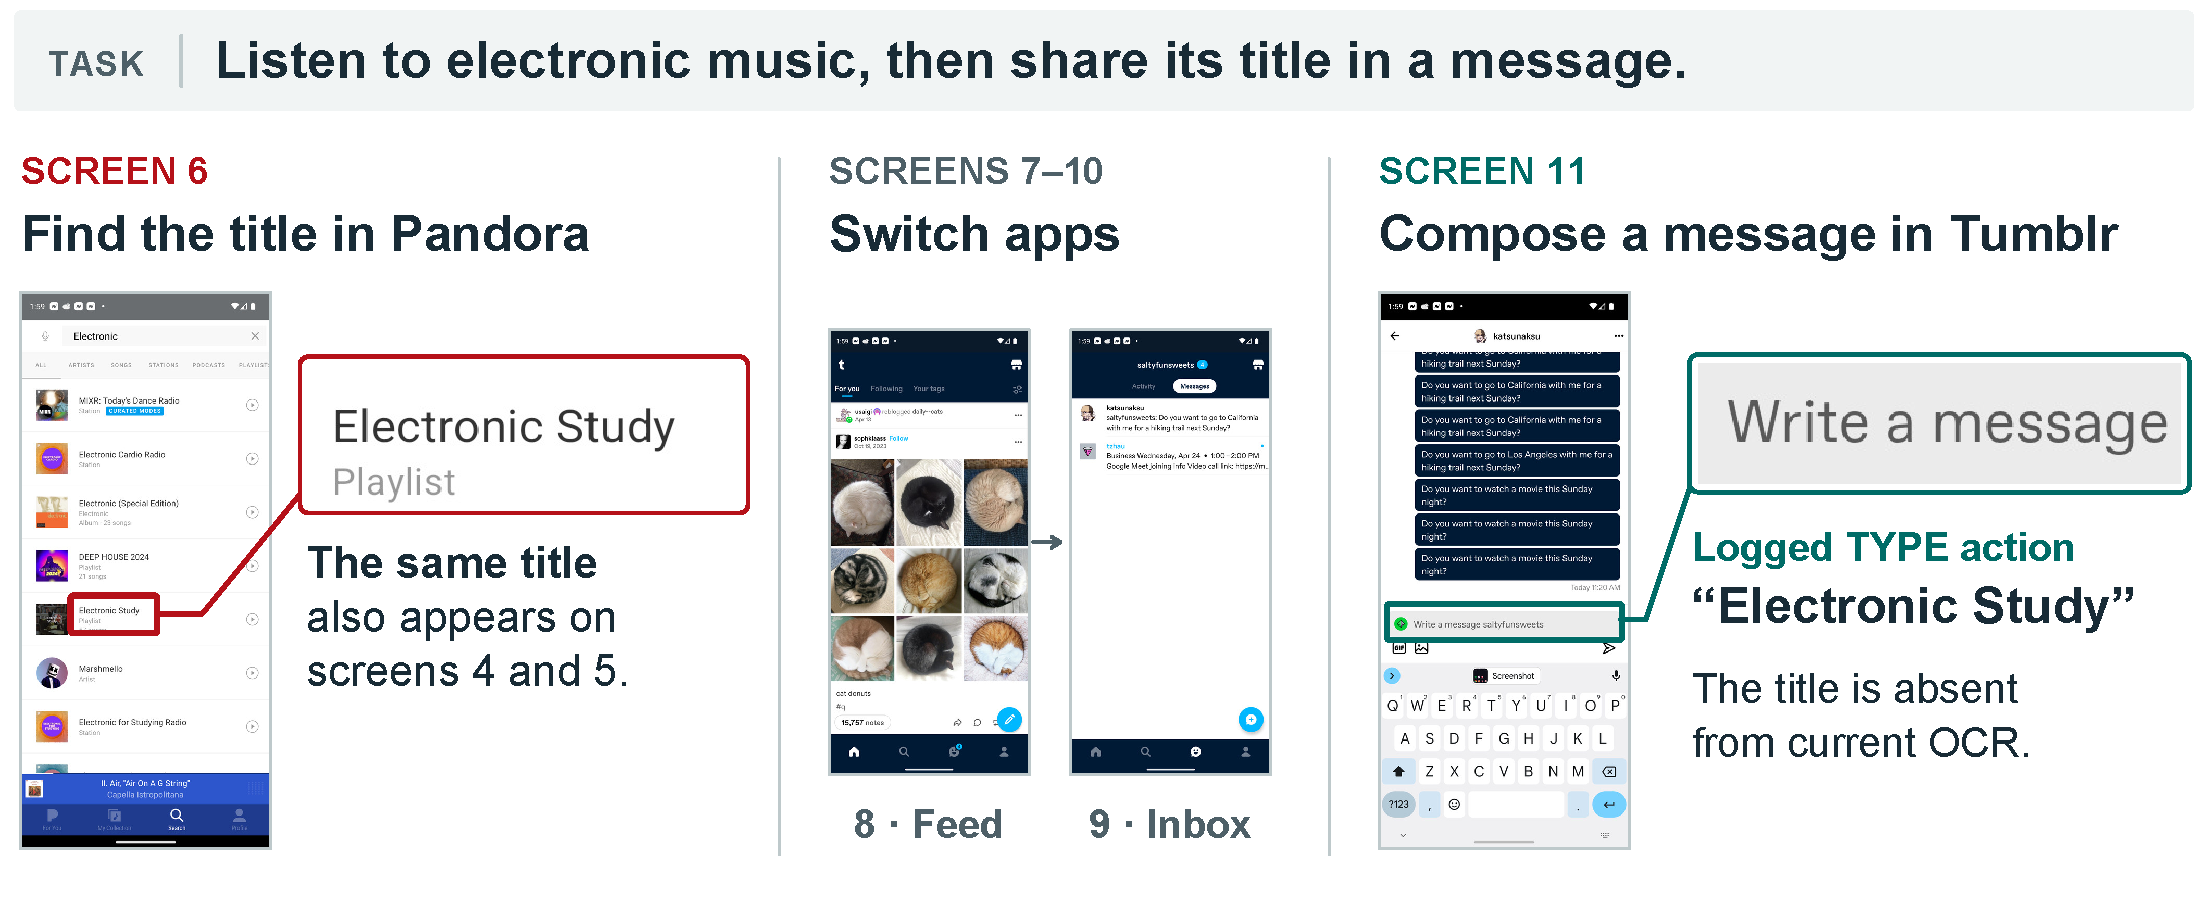
\includegraphics[width=\linewidth]{figures/scenario.pdf}
\caption{A music title crosses an app boundary in GUI-Odyssey episode 4671561041722435. Screen 6 is the last of three valid sources before the typing action at step 11. The scorer selected screen 6 and the full-history selector selected screen 5. Both readers missed the target text. Screenshots cropped and annotated from the \href{https://huggingface.co/datasets/OpenGVLab/GUI-Odyssey}{GUI-Odyssey release}~\citep{odysseypub}, \href{https://creativecommons.org/licenses/by/4.0/}{CC BY 4.0}.}
\label{fig:case}\end{figure}

Existing approaches fall into three groups. The first places the entire history in the prompt. The target text must then compete for the model's attention with every menu item, button and message, and the history consumes more context as it grows. Long-context studies also find that models make poor use of information in the middle of their input and are easily misled by similar distractors~\citep{lost,ruler,haystacks}. The second writes a summary or note for each screen and retrieves through those summaries~\citep{readagent,memgpt,mobileagente}. Each summary is written before the agent knows what it will need, so the target text is easily dropped. Summarizers are also often designed or trained together with a specific agent; GUI-Rise, for instance, rewards its summaries by how well its own agent acts afterwards~\citep{guirise}, so a summarizer may not carry over to another agent or task. A recent third approach trains the agent to actively look back at earlier screenshots~\citep{palui}. Because ordinary demonstrations do not mark which screen to revisit, PAL-UI uses a stronger teacher model in a four-stage pipeline to synthesize 8.6K step-level examples, so its supervision is only as good as the teacher. Annotating these decisions by hand would be costly, since an annotator must read a whole trajectory to label a single decision.

Training an agent to look back, however, hinges on one missing label: at each text entry, which earlier screen holds the answer? We observe that this label can be read directly from a demonstration, because the demonstration records the text the user actually typed. In Figure~\ref{fig:case}, the log shows that the user typed \emph{Electronic Study} at step 11. We run OCR on every earlier screen and search each one for that string: screens 4, 5 and 6 contain it and the others do not, so screens 4, 5 and 6 are labeled as answer screens. Every logged text entry yields labels in this way, without human annotation or a teacher model. With these labels, we train a model to find such a screen without knowing the answer. At test time the model never sees the typed text; it must decide which screen to revisit from the task description, the current screen and the earlier screens. The selected screen is then marked and passed to a reader, which writes the text to type.

\paragraph{Contributions.}
\begin{enumerate}\setlength{\itemsep}{2pt}
\item \textbf{We verify that prompting alone does not reliably find the source screen.} On 188 typing steps from GUI-Odyssey, an untrained 7B per-screen model finds a valid source in 50.0\% of cases, a 14B full-history prompt in 54.8\% and a summary-based screen index in 41.0\%. The task becomes harder later in a trajectory: the full-history prompt finds 68.0\% of sources at steps $t\leq15$ but only 46.0\% at $t\geq16$.
\item \textbf{We solve the missing-label problem by deriving labels from demonstrations.} Matching the typed text against the OCR of every earlier screen turns 188 logged entries into 2,861 labeled case--screen pairs, with no human or teacher labels. We train two 7B selectors on them: one scores each earlier screen, and the other reads the whole history and outputs a screen number. With the base model, prompt and reader held fixed, training raises the per-screen model's localization from 50.0\% to 72.3\% and its typed-text accuracy from 35.1\% to 44.7\%.
\item \textbf{We evaluate extensively.} On 93 held-out cases from disjoint trajectories, the per-screen model's localization rises from 41.9\% to 79.6\%. We further compare two definitions of look-back distance and ablate both the selector and the reader. Together, these results validate look-back supervision that requires no human annotation.
\end{enumerate}

\section{Method}
\label{sec:method}
We study one typing decision at a time. At step $t$ of an episode, the agent knows that it must enter text that is not on the current screen; it must choose an earlier screen that shows the text and then produce the text. Its input is the task instruction $I$, the OCR text $O_t$ of the current screen and the OCR text of the earlier screens $O_0,\dots,O_{t-1}$, numbered in order. Figure~\ref{fig:method} shows how we derive training labels from a demonstration and how the two selectors use them at inference.

\begin{figure}[t]\centering
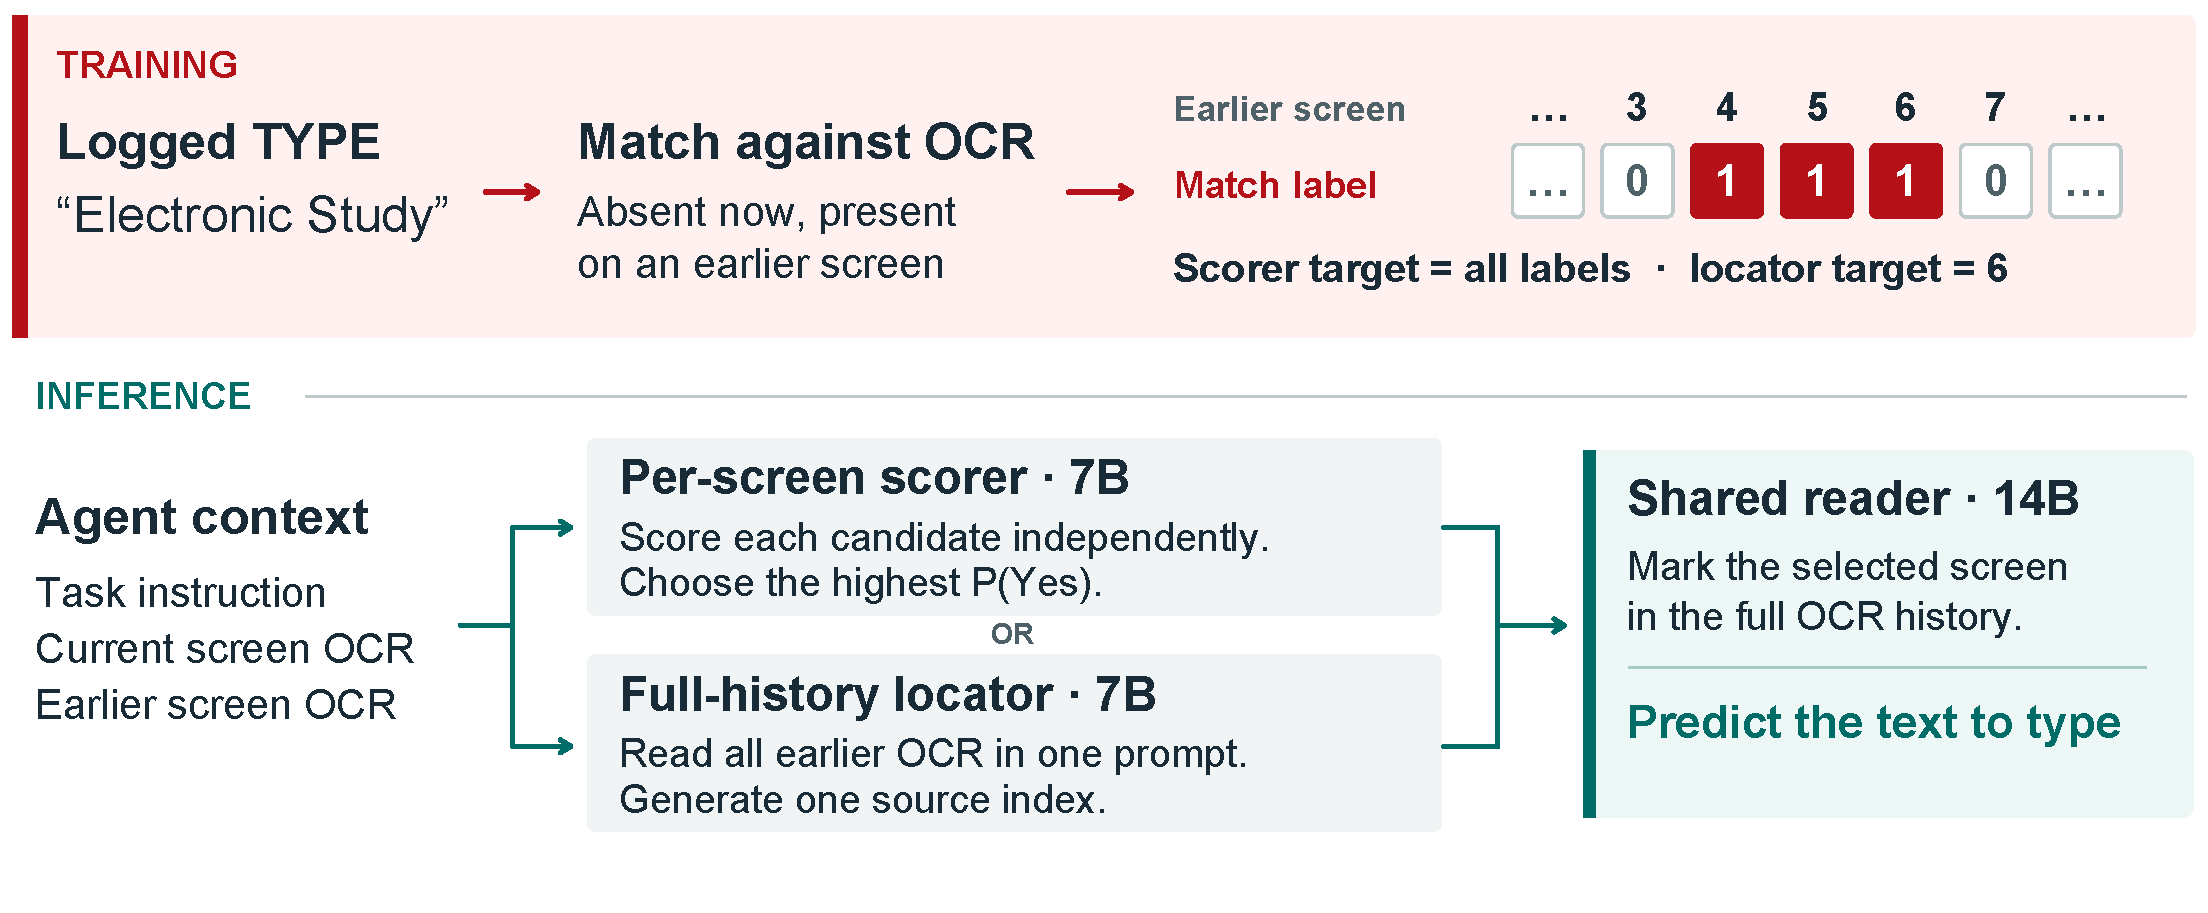
\includegraphics[width=\linewidth]{figures/method.pdf}
\caption{Verifier-supervised look-back. During training, the logged text entry is matched against the OCR of every earlier screen; the resulting source set labels each candidate for the per-screen scorer and gives the latest valid screen ID as the target of the full-history selector. At inference, either selector chooses a screen without seeing the logged text, and a shared reader receives the history with the selected screen marked and predicts the text to type.}
\label{fig:method}\end{figure}

\subsection{Deriving look-back labels from demonstrations}
\label{sec:labels}
Let $a_t$ be the text entered at step $t$ of a demonstration. We lowercase strings and remove whitespace and commas, including the Chinese comma, and write $m(a,O)=1$ when the normalized $a$ occurs as a substring of the normalized $O$. The set of valid source screens is
\[
V_t=\{\,i : 0\leq i<t,\; m(a_t,O_i)=1\,\}.
\]
A text entry becomes a case if $a_t$ has at least three normalized characters, $m(a_t,I)=0$, OCR is available for the current screen, $m(a_t,O_t)=0$ and $V_t$ is non-empty. The last two conditions keep only entries whose answer has left the screen but appeared earlier; Section~\ref{sec:filters} shows that dropping the current-screen condition can reverse a comparison. Every earlier screen with OCR then receives the label $y_{ti}=\mathbf{1}[i\in V_t]$. In Figure~\ref{fig:case}, a single logged entry labels screens 4, 5 and 6 as positives and every other earlier screen as a negative. The entered text $a_t$ is used only to build labels and to score predictions; neither the selector nor the reader sees it at test time.

\subsection{Selecting a source screen}
We train two selectors that differ only in how the history reaches the model. Both start from Qwen2.5-7B-Instruct~\citep{qwen} and add a rank-16 LoRA adapter~\citep{lora} on the attention projections.

\paragraph{Per-screen scorer.} The scorer judges one candidate at a time. For candidate $i$, its prompt contains $I$, $O_t$, $O_i$ (truncated to 1,200 characters) and the distance $t-i$, and it ends with a Yes/No question. We read the next-token logits of \texttt{Yes} and \texttt{No}, apply a two-way softmax to obtain $s_i=P(\texttt{Yes})$, and train with binary cross-entropy against $y_{ti}$, weighting positives by three. At inference, the scorer selects $\hat i=\arg\max_{i<t}s_i$. Because every earlier screen is a training item, the 188 development cases yield 2,861 case--screen pairs, of which 463 (16.2\%) are positive; these pairs share context within each of the 188 decisions.

\paragraph{Full-history selector.} The selector reads $I$, $O_t$ and the numbered history in one prompt, with each earlier screen truncated to 700 characters, and generates the index of a source screen. When several screens match, we train it to output the latest one, $\max V_t$, which gives a single target sequence. The loss covers only the target tokens, and inference decodes greedily for at most five tokens. Both selectors train for two epochs at learning rate $10^{-4}$, accumulating four items per update. The scorer runs one forward pass per candidate, about 12K input tokens in total at $t=16$, whereas the selector reads 1--5K tokens in a single pass.

\subsection{Reading the selected screen}
A frozen Qwen2.5-14B-Instruct reader generates the text to enter. Its prompt contains $I$, the OCR of all earlier screens, the selected screen repeated and marked, and $O_t$. Keeping the rest of the history lets the reader recover from an imperfect selection, while the mark tells it where to look first. The trained selectors and the untrained per-screen control share this reader and prompt, so their typed-text accuracies differ only through the selected screen. A single-screen variant, which sees only the selected screen, serves as a reading control.

\section{Experiments}
\subsection{Experimental setup}
\label{sec:setup}
\paragraph{Data.} We use the first public release of GUI-Odyssey~\citep{odysseyv1}, which contains 7,735 cross-app trajectories; the later ICCV version describes an expanded release~\citep{odysseypub}. We run EasyOCR on the screenshots of four sampled batches and mine cases as described in Section~\ref{sec:labels} (Table~\ref{tab:data}). The first batch samples trajectories that contain a candidate entry, the second and third target later steps, and the fourth takes trajectories of at least 16 steps with a candidate at $t\geq12$ while excluding all earlier batches. The first three batches form a development pool of 188 cases from 182 trajectories. We split it into five folds of 36--40 cases, keeping all cases of a trajectory in the same fold, train on four folds and predict the fifth; every development number below pools the five out-of-fold predictions. The fourth batch is a held-out set of 93 cases from 90 trajectories that share no episode with the development pool. For it, each selector is trained once on all 188 development cases and evaluated once. Most held-out cases occur at moderately late steps: 72 at $t=12$--15, 19 at $t=16$--19 and two at $t\geq20$.

\begin{table}[!htb]\centering
\caption{Sampling and case retention. Used trajectories are distinct episodes that contribute at least one retained case. The first three batches form the development pool.}
\label{tab:data}\small
\begin{tabular}{lrrrr}\toprule
Batch & Sampled trajectories & Candidate entries & Cases & Used trajectories\\\midrule
First & 300 & 431 & 85 & 81\\
Long & 300 & 355 & 53 & 53\\
Later-mined & 200 & 252 & 50 & 48\\\midrule
Development total & 800 & 1,038 & 188 & 182\\
Held-out batch & 400 & 438 & 93 & 90\\\bottomrule
\end{tabular}\end{table}

\paragraph{Baselines.} We compare the trained selectors with three prompted ones. The \emph{untrained per-screen} model uses the scorer's base model and prompt without the adapter, which isolates the effect of training. The \emph{full-history prompt} gives Qwen2.5-14B-Instruct the numbered history and asks for the source screen. The \emph{screen index}, inspired by ReadAgent~\citep{readagent}, has Qwen2.5-7B-Instruct write a one-line note of at most 20 words for every screen, naming the kind of screen and the kinds of values it shows but not the values themselves; the 14B model then picks a screen from these notes and reads its full OCR.

\paragraph{Metrics.} \emph{Localization} is the fraction of cases with $\hat i\in V_t$, so any screen that shows the answer counts as correct. \emph{Typed-text accuracy} is the fraction of cases in which the normalized generation contains the normalized reference text; periods are also removed for this check. A reader can pick the wrong field from a valid screen or recover the text from elsewhere in the history, so the two metrics capture different errors. All comparisons are paired on the same cases. We use two-sided McNemar tests with continuity correction and report nominal $p$-values from a single run per condition.

\subsection{Main results}
\label{sec:main}
Table~\ref{tab:main} reports localization and typed-text accuracy on the development pool and on the held-out set.

\begin{table}[t]\centering
\caption{Source-screen localization and typed-text accuracy (\%). The two 7B per-screen rows share the inference prompt and the reader. A dash marks a result that was not measured.}
\label{tab:main}\small
\begin{tabular}{lrrrr}\toprule
& \multicolumn{2}{c}{Development ($n=188$)}&\multicolumn{2}{c}{Held out ($n=93$)}\\
\cmidrule(lr){2-3}\cmidrule(lr){4-5}
Selector & Localization & Typed text & Localization & Typed text\\\midrule
Prompted screen index (14B) &41.0 &23.9 &37.6 &18.3\\
Prompted full history (14B) &54.8 &31.4 &59.1 &23.7\\
Untrained per-screen (7B) &50.0 &35.1 &41.9 & --\\\midrule
Trained full history (7B) &65.4 &42.6 &76.3 &\textbf{51.6}\\
Trained per-screen (7B) &\textbf{72.3} &\textbf{44.7} &\textbf{79.6} &49.5\\\bottomrule
\end{tabular}\end{table}

\paragraph{Derived labels make the per-screen model a much better selector.} With the base model, prompt and reader held fixed, training raises the scorer's development localization from 50.0\% to 72.3\%: 52 cases change from wrong to right and 10 from right to wrong ($p<0.001$). The same reader then types the correct text in 84 instead of 66 cases (23 gains and five losses, $p=0.0013$). On the held-out set, localization rises from 41.9\% to 79.6\%, so the gain carries over to unseen trajectories from the same corpus.

\paragraph{Both trained selectors outperform prompting.} The trained full-history selector localizes 123 of 188 development sources, compared with 103 for the 14B full-history prompt ($p=0.019$), although it uses a smaller model. On the held-out set, the scorer, the trained full-history selector and the full-history prompt localize 74, 71 and 55 of 93 sources, and the scorer's margin over the prompt is significant ($p=0.003$). The typed-text gaps to this baseline are larger but partly reflect the reading protocol, because the baseline's reader saw unmarked history in the first batch and only the selected screen elsewhere. A cleaner reading comparison keeps the trained scorer fixed and adds history to the reader, which raises held-out typed-text accuracy from 37.6\% to 49.5\% ($p=0.016$).

\paragraph{The two trained selectors are statistically close.} With a shared reader, the scorer finds 13 more development sources than the full-history selector ($p=0.086$) and types four more correct entries ($p=0.45$); on the held-out set the difference is three localizations ($p=0.63$). Both architectures benefit from the same labels, and the remaining difference between them is not statistically reliable.

\paragraph{Later steps are harder, and training narrows the drop.} At early steps ($t\leq15$, 75 cases), the full-history prompt, the trained full-history selector and the trained scorer localize 68.0\%, 76.0\% and 80.0\% of sources. At $t\geq16$ (113 cases), they localize 46.0\%, 58.4\% and 67.3\%. The step index counts the screens before the entry rather than the distance to the evidence, which we analyze in Section~\ref{sec:distance}.

\subsection{Finding the screen is not the same as reading it}
\label{sec:reading}
On the development pool, 74 of the scorer's 136 correct selections also yield the correct text, while in the other 62 the reader misses the value on a valid screen. Conversely, the reader recovers the text in 10 of the 52 cases with an invalid selection, because the unmarked history remains in its context. The held-out set shows the same pattern, with 43 of 74 correct selections yielding the right text and three recoveries after an invalid selection. The reader controls in Table~\ref{tab:controls} (right) show that reading is now the bottleneck: marking a screen known to be valid adds only one correct entry over the scorer's own choice (85 versus 84), whereas marking the most recent or a random earlier screen lowers accuracy to 38.8\% and 36.7\%. The reader must find the task-relevant field among many strings on a screen and copy it exactly. In Figure~\ref{fig:case}, both selectors chose valid screens, yet both readers missed the title.

\subsection{How far back does the model look?}
\label{sec:distance}
The answer recurs on several screens in 111 of the 188 development cases, so look-back distance has two natural definitions: the distance to the earliest match, $g_{\rm first}=t-\min V_t$, and the shortest sufficient look-back, $g_{\rm recent}=t-\max V_t$. Their medians are seven and four screens, and in Figure~\ref{fig:case} they are seven and five. Figure~\ref{fig:distance} partitions the same predictions under both definitions.

\begin{figure}[t]\centering
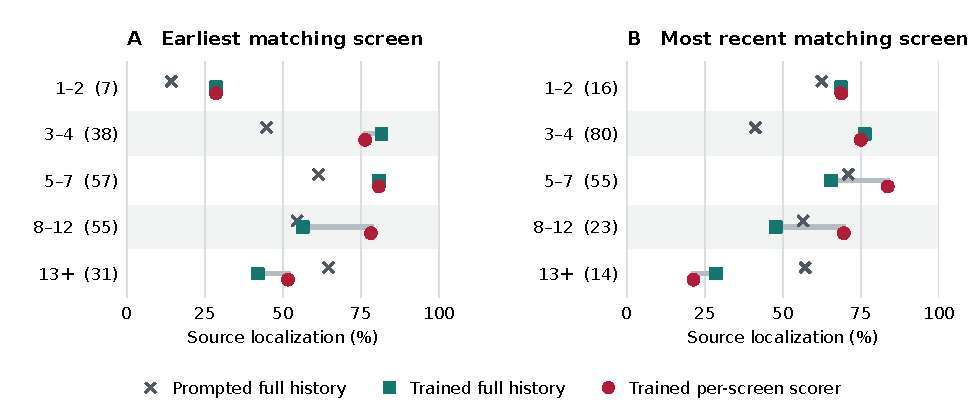
\includegraphics[width=\linewidth]{figures/distance.pdf}
\caption{Source localization by distance to the first (A) or the most recent (B) matching screen. Rows give distance ranges with case counts in parentheses. Both panels partition the same 188 development predictions.}
\label{fig:distance}\end{figure}

Grouped by $g_{\rm first}$, the scorer's advantage concentrates at 8--12 screens, where it finds 43 of 55 sources against 31 for the trained full-history selector (78.2\% versus 56.4\%; 13 improvements and one regression, $p=0.003$). Grouped by $g_{\rm recent}$, the same band holds only 23 cases and the difference (69.6\% versus 47.8\%) is not significant ($p=0.131$), because many cases with old earliest evidence also contain a recent copy (17 of the 31 cases with $g_{\rm first}\geq13$). On the 14 cases whose most recent evidence is at least 13 screens old, the full-history prompt finds eight sources, the trained full-history selector four and the scorer three. These groups are too small to support a precise cutoff for choosing between selectors, but they show that conclusions about distance depend on which occurrence is measured.

\subsection{Ablations and evaluation filters}
\label{sec:filters}
\begin{table}[t]\centering
\caption{Controlled variations on the 188 development cases. The left half changes the per-screen selector; the right half changes which screen the same reader sees marked in the history.}
\label{tab:controls}\small
\begin{tabular}{lr@{\hspace{1.4em}}lr}\toprule
Selector variation & Loc. (\%) & Reader highlight & Text (\%)\\\midrule
7B, distance, weight 3 &72.3 & Scorer's top screen &44.7\\
Omit distance header &70.7 & Scorer's top two screens &45.2\\
Positive weight 1 &72.3 & Known valid screen &45.2\\
Smaller 3B model &68.1 & Most recent screen &38.8\\
 & & Random earlier screen &36.7\\\bottomrule
\end{tabular}\end{table}

\paragraph{Selector ablations.} The left half of Table~\ref{tab:controls} varies the scorer. Removing the explicit distance from the prompt changes localization by 1.6 points ($p=0.61$), and equal class weights leave it unchanged, so the result is not sensitive to these choices. A 3B scorer finds fewer sources overall (68.1\%) but more at $t\geq20$, where it reaches 48.1\% (13 of 27) against 37.0\% for the 7B scorer.

\paragraph{Why a screen index falls short.} In the example of Figure~\ref{fig:case}, the notes for screens 4, 5 and 6 list only kinds of values (\emph{name, url, station, playlist, \ldots}) and never the title itself. On the first 85 cases, the prompted one-line-per-screen index localizes 49.4\% of sources, compared with 65.9\% for prompting with the full OCR. Training the line writer with preference optimization does not close this gap (45.9\%), even though its preference pairs reuse the evaluation set, and four writer variants range from 43.5\% to 49.4\%. A BM25 retriever queried with the task and the current screen finds 10.6\% of sources but 92.9\% when queried with the hidden answer, which shows that the difficulty lies in not knowing what to search for.

\paragraph{Two evaluation filters change conclusions.} First, 40 of the first 85 cases have several valid screens; crediting only the earliest one would understate the screen index by 15.3 points and the full-history prompt by 11.8. Second, cases whose answer is still on the current screen reward any method that reads recent screens. On the unfiltered 127-case long batch, a recent-screen gating rule beat the full-history prompt by 17.3 points, but after removing the 74 leaked cases it trailed by 22.7 points on the remaining 53, and we withdrew that earlier finding.

\section{Related work}
\paragraph{GUI agents and datasets.} Large demonstration corpora such as AITW~\citep{aitw} and AndroidControl~\citep{androidcontrol} pair natural-language instructions with screen--action sequences. AITZ~\citep{aitz} and AMEX~\citep{amex} add screen descriptions, action rationales and element-function annotations, and GUI-Odyssey~\citep{odysseypub} collects longer cross-app tasks. AndroidWorld~\citep{androidworld} instead runs tasks on a live device and checks the final system state. On the modeling side, Auto-GUI~\citep{autogui} predicts the next action from the screen and the previous actions; CogAgent~\citep{cogagent}, SeeClick~\citep{seeclick} and OS-Atlas~\citep{osatlas} train on large-scale GUI grounding data to locate interface elements; and UI-TARS~\citep{uitars} maps screenshots to actions end to end. These works mainly address where to act on the current screen. We study a different kind of localization, in which the answer is no longer on the current screen and the agent must find the earlier screen that shows it.

\paragraph{History and memory in GUI agents.} Many agents keep the history as a textual action sequence~\citep{autogui} or compress past screenshots; GUI-Odyssey's OdysseyAgent, for example, resamples historical screenshot features~\citep{odysseypub}. Other agents record information while they act: Mobile-Agent-v2~\citep{mobileagentv2} has a decision agent update a memory unit of task-relevant content, Mobile-Agent-E~\citep{mobileagente} uses a notetaker agent to record important information, and GUI-Rise~\citep{guirise} writes a history summary at every step and trains it with a reward tied to later actions. All of them decide what to keep when a screen is first seen, before the agent knows which field it will need. Cross-episode memories, such as AppAgent's exploration documents~\citep{appagent}, Synapse's exemplar trajectories~\citep{synapse} and the reusable workflows of Agent Workflow Memory~\citep{awm}, store how to perform tasks rather than what the current episode showed. Closest to our work is PAL-UI~\citep{palui}, which summarizes the history and trains an agent to retrieve an earlier screenshot when needed. Its 8.6K step-level examples are synthesized by a teacher model and supervise both when to look back and which frame to retrieve. We isolate the second decision and supervise it with the text recorded in the demonstration, so any corpus that logs typed text can supply training data.

\paragraph{Long-context and multi-image retrieval.} Lost in the Middle~\citep{lost} finds that language models make poor use of information in the middle of long inputs. RULER~\citep{ruler} shows that simple needle-in-a-haystack tests overstate the context length that models can actually use, and Visual Haystacks~\citep{haystacks} extends the question to large image collections, finding that models are misled by visual distractors and show a positional bias. ReadAgent~\citep{readagent} and MemGPT~\citep{memgpt} work within a limited context by retrieving original content through gists or a hierarchical memory. Our histories span only 1--5K tokens, so a full-history prompt remains feasible. The answer, however, often recurs across screens, which makes look-back distance ambiguous; Section~\ref{sec:distance} therefore reports the distance to both the earliest and the most recent occurrence.

\paragraph{Distant supervision from known answers.} Distant supervision was introduced for relation extraction, where facts in a knowledge base label sentences automatically~\citep{mintz}. Open-domain question answering adopted the idea: DrQA~\citep{drqa} trains its reader on retrieved paragraphs that contain the answer string, ORQA~\citep{orqa} learns a retriever and a reader jointly from question--answer pairs alone, and DPR~\citep{dpr} uses BM25 passages that contain the answer as retriever positives when no gold passage is given. We bring this idea to GUI trajectories. The typed text plays the role of the answer and the screens before the current step bound the search, so we can check every earlier screen and keep all matches rather than only the top-ranked one. Our two selectors also mirror the two common reranking formulations: the per-screen scorer scores each candidate independently, as monoT5~\citep{monot5} does with the probabilities of \texttt{true} and \texttt{false}, while the full-history selector compares all candidates in one prompt, as RankGPT~\citep{rankgpt} does. A match, however, only shows that a screen contains the text; picking the right field on that screen remains a separate reading problem.

\section{Code and reproduction}
All code, derived data and per-case predictions are released in the \href{https://github.com/WMSlalalala/verifier-supervised-lookback}{project repository}. Its \texttt{src/} directory holds the scripts that sample GUI-Odyssey trajectories, run OCR and verify cases, build the case--screen labels (\texttt{build\_scorer\_data.py}), train the two selectors (\texttt{train\_scorer.py} and \texttt{train\_fullhist.py}) and run the reader (\texttt{read\_scorer.py}), together with the analysis scripts behind every table and figure. EasyOCR provides text recognition, and Transformers and PEFT run the Qwen2.5 models and their LoRA adapters.

Because the OCR records, labels and predictions are released in \texttt{data/} and \texttt{results/}, the main numbers can be recomputed on a CPU without the original screenshots or model weights. The snippet below uses only the Python standard library and prints 188/123/80, 188/136/84, 93/71/48 and 93/74/46 (cases, correct screens, correct typed text) for the trained full-history selector and the scorer on the development and held-out sets, matching Table~\ref{tab:main}.
\begin{lstlisting}[language=Python]
import json
from pathlib import Path
for split in ("", "_more"):
    for model in ("fullhist", "scorer"):
        path = Path("results") / f"{model}_trained{split}_hist_e2e.json"
        rows = json.loads(path.read_text(encoding="utf-8"))
        print(model, len(rows), sum(r["loc"] for r in rows),
              sum(r["e2e"] for r in rows))
\end{lstlisting}
Retraining both selectors over the five folds and running the reader needs a CUDA GPU (the reported 7B runs used a 48~GB card); for the held-out set, set \texttt{FOLD=ext} for the trainers and \texttt{SET=\_more} for the reader. The repository README lists the remaining commands and maps each table and figure in this report to the files that produce it.
\begin{lstlisting}[language=bash]
mkdir -p run-data && cp data/*.json* results/*.json run-data/
bash configure.sh "$PWD/run-data"
for f in 0 1 2 3 4; do
  FOLD=$f python src/train_scorer.py
  FOLD=$f python src/train_fullhist.py
done
for model in scorer fullhist; do
  PREFIX=$model SRC=trained HIST=1 python src/read_scorer.py
done
\end{lstlisting}

\section{Conclusion and limitations}
A recorded text entry already tells us which earlier screens hold the answer. Using these matches as labels, without human annotation or a teacher model, a 7B per-screen scorer finds the source screen in 72.3\% of development cases instead of 50.0\% and in 79.6\% of held-out cases instead of 41.9\%, and a full-history selector trained on the same labels performs comparably. Reading remains the bottleneck: the reader still misses the value in 62 of the scorer's 136 correct selections.

Our evidence has four main limitations. All four samples come from one corpus and one OCR engine. A substring can match by coincidence, and OCR errors or paraphrases can hide genuine matches. A 20-case spot check found the target visible on every inspected source screen, and in five of these cases the user had typed it earlier; this supports the presence of visible evidence but says little about whether users actually needed to remember the value. Finally, localization uses the same criterion that creates the labels, typed-text accuracy accepts the reference as a substring of a longer generation, and neither metric measures whole-task success.

\begingroup\small\setlength{\bibsep}{2pt}
\begin{thebibliography}{32}
\bibitem{appagent} C. Zhang, Z. Yang, J. Liu, Y. Han, X. Chen, Z. Huang, B. Fu and G. Yu. \href{https://arxiv.org/abs/2312.13771}{AppAgent: Multimodal Agents as Smartphone Users}. CHI, 2025.
\bibitem{mobileagentv2} J. Wang, H. Xu, H. Jia, X. Zhang, M. Yan, W. Shen, J. Zhang, F. Huang and J. Sang. \href{https://proceedings.neurips.cc/paper_files/paper/2024/hash/0520537ba799d375b8ff5523295c337a-Abstract-Conference.html}{Mobile-Agent-v2: Mobile Device Operation Assistant with Effective Navigation via Multi-Agent Collaboration}. NeurIPS, 2024.
\bibitem{uitars} Y. Qin et al. \href{https://arxiv.org/abs/2501.12326}{UI-TARS: Pioneering Automated GUI Interaction with Native Agents}. arXiv:2501.12326, 2025.
\bibitem{aitw} C. Rawles, A. Li, D. Rodriguez, O. Riva and T. Lillicrap. \href{https://arxiv.org/abs/2307.10088}{Android in the Wild: A Large-Scale Dataset for Android Device Control}. NeurIPS Datasets and Benchmarks Track, 2023.
\bibitem{androidcontrol} W. Li et al. \href{https://arxiv.org/abs/2406.03679}{On the Effects of Data Scale on UI Control Agents}. NeurIPS Datasets and Benchmarks Track, 2024.
\bibitem{odysseypub} Q. Lu, W. Shao, Z. Liu, L. Du, F. Meng, B. Li, B. Chen, S. Huang, K. Zhang and P. Luo. \href{https://openaccess.thecvf.com/content/ICCV2025/html/Lu_GUIOdyssey_A_Comprehensive_Dataset_for_Cross-App_GUI_Navigation_on_Mobile_ICCV_2025_paper.html}{GUIOdyssey: A Comprehensive Dataset for Cross-App GUI Navigation on Mobile Devices}. ICCV, 2025.
\bibitem{lost} N. F. Liu, K. Lin, J. Hewitt, A. Paranjape, M. Bevilacqua, F. Petroni and P. Liang. \href{https://aclanthology.org/2024.tacl-1.9/}{Lost in the Middle: How Language Models Use Long Contexts}. TACL, 12:157--173, 2024.
\bibitem{ruler} C.-P. Hsieh et al. \href{https://arxiv.org/abs/2404.06654}{RULER: What's the Real Context Size of Your Long-Context Language Models?} COLM, 2024.
\bibitem{haystacks} T.-H. Wu, G. Biamby, J. Quenum, R. Gupta, J. E. Gonzalez, T. Darrell and D. M. Chan. \href{https://arxiv.org/abs/2407.13766}{Visual Haystacks: A Vision-Centric Needle-In-A-Haystack Benchmark}. ICLR, 2025.
\bibitem{readagent} K.-H. Lee, X. Chen, H. Furuta, J. Canny and I. Fischer. \href{https://proceedings.mlr.press/v235/lee24c.html}{A Human-Inspired Reading Agent with Gist Memory of Very Long Contexts}. ICML, 2024.
\bibitem{memgpt} C. Packer, S. Wooders, K. Lin, V. Fang, S. G. Patil, I. Stoica and J. E. Gonzalez. \href{https://arxiv.org/abs/2310.08560}{MemGPT: Towards LLMs as Operating Systems}. arXiv:2310.08560, 2023.
\bibitem{mobileagente} Z. Wang et al. \href{https://arxiv.org/abs/2501.11733}{Mobile-Agent-E: Self-Evolving Mobile Assistant for Complex Tasks}. arXiv:2501.11733, 2025.
\bibitem{guirise} T. Liu, C. Wang, R. Li, Y. Yu, X. He and S. Bai. \href{https://papers.nips.cc/paper_files/paper/2025/hash/f144ab9985c739a5091ec188a2688644-Abstract-Conference.html}{GUI-Rise: Structured Reasoning and History Summarization for GUI Navigation}. NeurIPS, 2025.
\bibitem{palui} Z. Liu, J. Li, W. X. Zhao, D. Gao, Y. Li and J.-R. Wen. \href{https://aclanthology.org/2026.findings-aacl.13/}{PAL-UI: Planning with Active Look-back for Vision-Based GUI Agents}. Findings of IJCNLP-AACL, 2026.
\bibitem{qwen} Qwen Team. \href{https://arxiv.org/abs/2412.15115}{Qwen2.5 Technical Report}. arXiv:2412.15115, 2024.
\bibitem{lora} E. J. Hu, Y. Shen, P. Wallis, Z. Allen-Zhu, Y. Li, S. Wang, L. Wang and W. Chen. \href{https://openreview.net/pdf?id=nZeVKeeFYf9}{LoRA: Low-Rank Adaptation of Large Language Models}. ICLR, 2022.
\bibitem{odysseyv1} Q. Lu et al. \href{https://arxiv.org/abs/2406.08451v1}{GUI Odyssey: A Comprehensive Dataset for Cross-App GUI Navigation on Mobile Devices}. arXiv:2406.08451v1, 2024. Initial dataset release.
\bibitem{aitz} J. Zhang et al. \href{https://aclanthology.org/2024.findings-emnlp.702/}{Android in the Zoo: Chain-of-Action-Thought for GUI Agents}. Findings of EMNLP, 2024.
\bibitem{amex} Y. Chai et al. \href{https://aclanthology.org/2025.findings-acl.110/}{AMEX: Android Multi-annotation Expo Dataset for Mobile GUI Agents}. Findings of ACL, 2025.
\bibitem{androidworld} C. Rawles et al. \href{https://proceedings.iclr.cc/paper_files/paper/2025/hash/01a83bc2f2732a58e6aa731e659e7101-Abstract-Conference.html}{AndroidWorld: A Dynamic Benchmarking Environment for Autonomous Agents}. ICLR, 2025.
\bibitem{autogui} Z. Zhang and A. Zhang. \href{https://aclanthology.org/2024.findings-acl.186/}{You Only Look at Screens: Multimodal Chain-of-Action Agents}. Findings of ACL, 2024.
\bibitem{cogagent} W. Hong et al. \href{https://openaccess.thecvf.com/content/CVPR2024/html/Hong_CogAgent_A_Visual_Language_Model_for_GUI_Agents_CVPR_2024_paper.html}{CogAgent: A Visual Language Model for GUI Agents}. CVPR, 2024.
\bibitem{seeclick} K. Cheng et al. \href{https://aclanthology.org/2024.acl-long.505/}{SeeClick: Harnessing GUI Grounding for Advanced Visual GUI Agents}. ACL, 2024.
\bibitem{osatlas} Z. Wu et al. \href{https://proceedings.iclr.cc/paper_files/paper/2025/hash/0faa4bc5f522076947a030273629d4fe-Abstract-Conference.html}{OS-ATLAS: Foundation Action Model for Generalist GUI Agents}. ICLR, 2025.
\bibitem{synapse} L. Zheng, R. Wang, X. Wang and B. An. \href{https://proceedings.iclr.cc/paper_files/paper/2024/hash/52f050499cf82fa8efb588e263f6f3a7-Abstract-Conference.html}{Synapse: Trajectory-as-Exemplar Prompting with Memory for Computer Control}. ICLR, 2024.
\bibitem{awm} Z. Z. Wang, J. Mao, D. Fried and G. Neubig. \href{https://proceedings.mlr.press/v267/wang25bx.html}{Agent Workflow Memory}. ICML, 2025.
\bibitem{mintz} M. Mintz, S. Bills, R. Snow and D. Jurafsky. \href{https://aclanthology.org/P09-1113/}{Distant Supervision for Relation Extraction without Labeled Data}. ACL-IJCNLP, 2009.
\bibitem{drqa} D. Chen, A. Fisch, J. Weston and A. Bordes. \href{https://aclanthology.org/P17-1171/}{Reading Wikipedia to Answer Open-Domain Questions}. ACL, 2017.
\bibitem{orqa} K. Lee, M.-W. Chang and K. Toutanova. \href{https://aclanthology.org/P19-1612/}{Latent Retrieval for Weakly Supervised Open Domain Question Answering}. ACL, 2019.
\bibitem{dpr} V. Karpukhin, B. Oguz, S. Min, P. Lewis, L. Wu, S. Edunov, D. Chen and W.-t. Yih. \href{https://aclanthology.org/2020.emnlp-main.550/}{Dense Passage Retrieval for Open-Domain Question Answering}. EMNLP, 2020.
\bibitem{monot5} R. Nogueira, Z. Jiang, R. Pradeep and J. Lin. \href{https://aclanthology.org/2020.findings-emnlp.63/}{Document Ranking with a Pretrained Sequence-to-Sequence Model}. Findings of EMNLP, 2020.
\bibitem{rankgpt} W. Sun et al. \href{https://aclanthology.org/2023.emnlp-main.923/}{Is ChatGPT Good at Search? Investigating Large Language Models as Re-Ranking Agents}. EMNLP, 2023.
\end{thebibliography}
\endgroup

\end{document}
